\subsubsection{OpenNI 2} OpenNI or Open Natural Interaction \cite{11} is a framework by the company PrimeSense and open source software project focused on improving interoperability of natural user interfaces for Natural Interaction (NI) devices, applications which use those devices and middleware that facilitates access and use of such devices. Microsoft Kinect and Asus Xtion are commercially available depth cameras which are compatible with OpenNI.

The OpenNI 2.0 API provides access to PrimeSense compatible depth sensors. It allows an application to initialize a sensor and receive depth, RGB and video streams from the device. OpenNI also provides a uniform interface that third party middleware developers can use to interact with depth sensors. Applications are then able to make use of both the third party middleware, as well as underlying basic depth and video data provided directly by OpenNI.

\subsubsection{NiTE 2} \label{sec:nite} PrimeSense Natural Interaction Technology for End-user (NiTE) \cite{12} is the middleware that perceives the world in 3D, based on the PrimeSensor depth images, and translates these perceptions into meaningful data in the same way as people do. NiTE middleware includes computer vision algorithms that enable identifying users and tracking their movements. Figure shows the architecture of NiTE, how it is working together with OpenNI, depth sensors and applications.

Figure \ref{fg:ni:arch} displays a layered view of producing, acquiring and processing depth data, up to the level of the application that utilizes it to form a natural- interaction based module. 

\begin{figure}
	[h] \centering 
	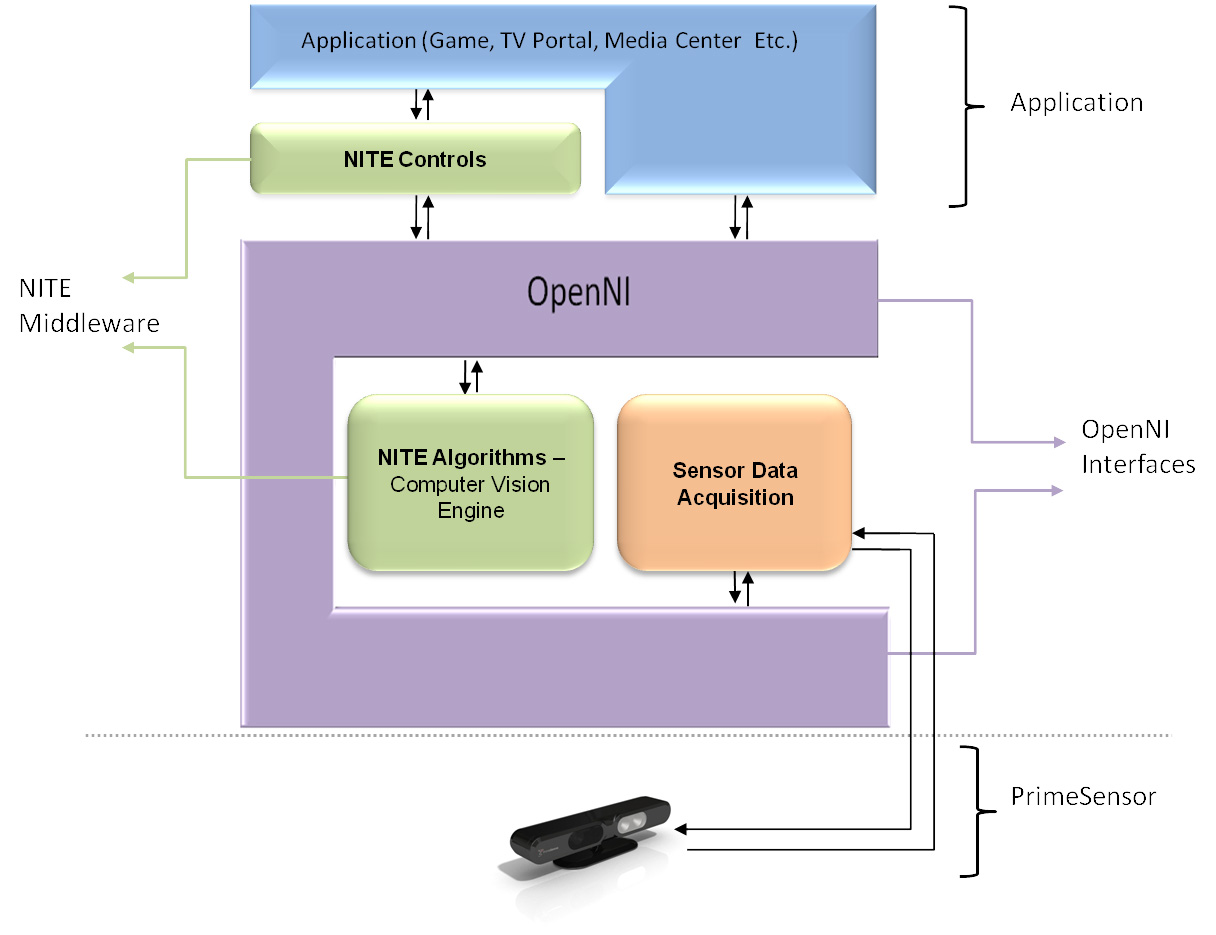
\includegraphics[height=10cm]{figures/content/ni-arch.jpg} \caption{NiTE Architecture} \label{fg:ni:arch} 
\end{figure}


\begin{itemize}
	\item The lower layer is the PrimeSensor device, that is the physical acquisition layer, resulting in raw sensory data from a stream of depth images. 
	\item The next C shaped layer is executed on the host PC represents OpenNI. OpenNI provides communication interfaces that interact with both the sensors driver and the middleware components, which analyze the data from the sensor. 
	\item The sensor data acquisition is a simple acquisition API, enabling the host to operate the sensor. This module is OpenNI compliant interfaces that conforms to OpenNI API standard. 
	\item The NiTE Algorithms layer is the computer vision middleware and is also plugged into OpenNI. It processes the depth images produced by the PrimeSensor. 
	\item The NiTE Controls layer is an applicative layer that provides application framework for gesture identification and gesture-based UI controls, on top of the data that is processed by NiTE Algorithms. 
\end{itemize}

\subsubsection{Skeletal Points Tracking Algorithm} The lower layer of NiTE middleware that performs the groundwork of processing the stream of raw depth images. This layer utilizes computer vision algorithms to perform the following: 
\begin{itemize}
	\item Scene segmentation is a process in which individual users and objects are separated from the background and tagged accordingly. 
	\item Hand point detection and tracking. 
	\item Full body tracking based on the scene segmentation output. Users bodies are tracked to output the current user pose with a set of locations of body joints. 
\end{itemize}

NiTE uses machine learning algorithms to recognize anatomical landmarks and pose of human body. Figure \ref{fg:ni:alg} shows how skeleton tracking algorithm works from a single input depth image and a per-pixel body part distribution is derived \cite{13}. Colors indicate the most likely part labels at each pixel and correspond to the joint proposals. Local modes of this signal are estimated to give high-quality proposals for the 3D locations of body joints, even for multiple users.

\begin{figure}
	[h] \centering 
	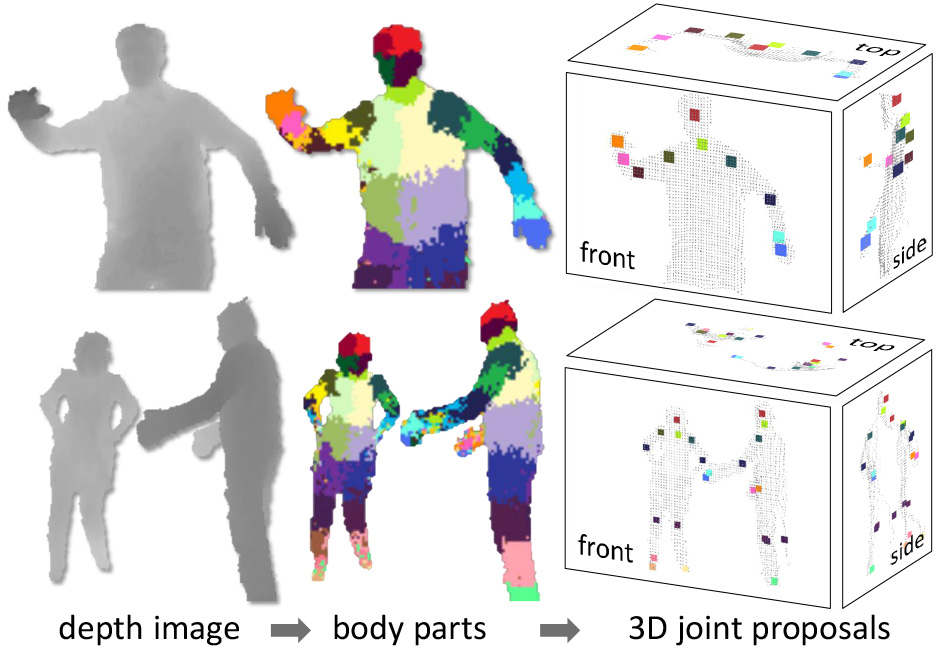
\includegraphics[height=8cm]{/content/ni-alg.jpg} \caption{Skeleton Tracking algorithm processes a depth image and a per-pixel body part distribution is inferred, and finally, 3D joints proposals are made for 15 points in human skeleton. \cite{13} } \label{fg:ni:alg} 
\end{figure}


\paragraph*{Training} In order to train the system, large collection of synthetic and real representations of human body are recorded and labeled. Each body representation is covered with several localized body part labels. Some of these parts are defined to directly localize particular skeletal joints of interest, while others fill the gaps or could be used in combination to predict other joints.

%\begin{figure}
	[h] \centering 
	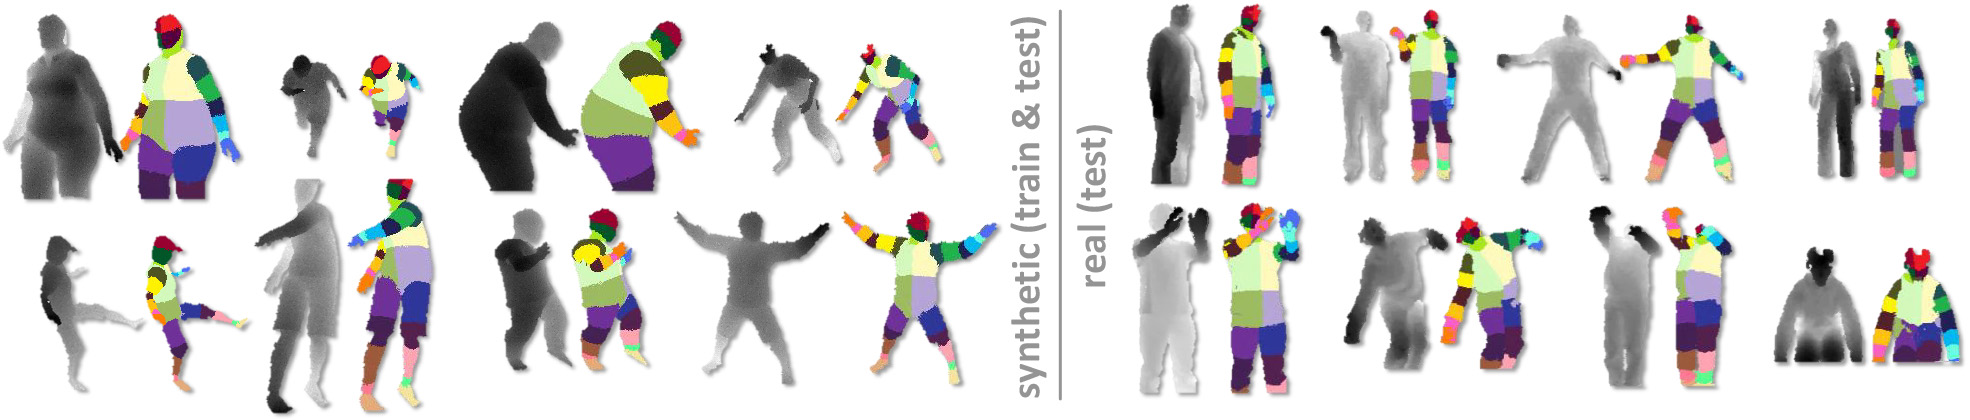
\includegraphics[height=3cm]{figures/content/ni-train.jpg} \caption{NiTE Synthetic and real training} \label{fg:ni:train} 
\end{figure}


\paragraph*{Feature Labeling} Features are located in depth image as shown in the figure \ref{fg:ni:label} and labeled. The yellow crosses indicates the pixel x being classified. The red circles indicate the offset pixel. In figure \ref{fg:ni:label} (a), the two example features $\theta_1, \theta_2$ give a large depth difference response. On the other hand in (b), the same two features at new image locations give a much smaller response.

\begin{figure}
	[h] \centering 
	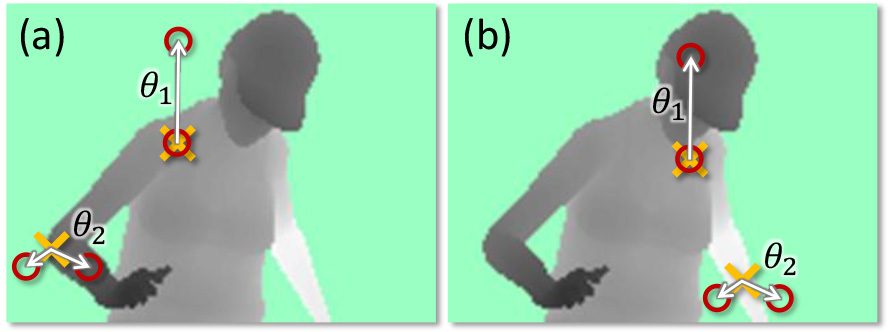
\includegraphics[height=4cm]{figures/content/ni-label.jpg} \caption{Features are located in depth image and labeled. \cite{2}} \label{fg:ni:label} 
\end{figure}


\paragraph*{Classification} Randomized decision forest is the classification algorithm to predict the probability of a pixel belonging to a body part. Randomized decision trees and forests have proven fast and effective multi-class classifiers for many tasks \cite{13}. Figure \ref{fg:ni:decision} shows the branching trees of Randomized Decision Forests algorithm and the red arrows indicate the different paths that might be taken by different trees for a particular input. A forest is an ensemble $T$ decision trees. Each tree consists of split nodes (blue) and leaf nodes (green). Each split node consists of a feature $f_\theta$ and a threshold $T$. 

\begin{figure}
	[h] \centering 
	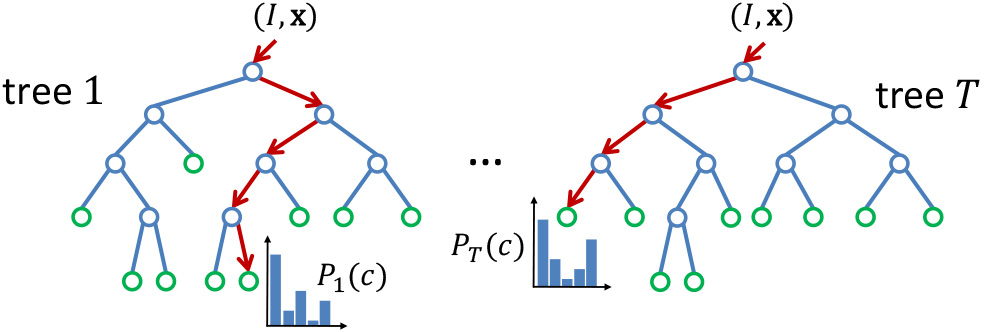
\includegraphics[height=4cm]{figures/content/ni-decision.jpg} \caption{Randomized decision forest} \label{fg:ni:decision} 
\end{figure}


\paragraph*{Prediction} To classify a pixel $x$ in image $I$ using Randomized decision tree, one starts at the root and repeatedly evaluates equation \ref{eq:ni:decision}, branching left or right according to the comparison of threshold {$ \tau$}. When the lead node in the decision treee $t$ is reached, a learned distribution $ P_t(c|I,x) $ over body part labels $c$ is stored. The distributions are averaged together for all trees in the forest to give the final classification.

\begin{equation}
\LARGE 
P_{t}(c|I,x) = \frac{1}{T} \sum_{t=1}^{T} P_{t}(c|I,x)
\label{eq:ni:decision}
\end{equation}

Each tree is trained on a different set of randomly synthesized images. A random subset of 2000 example pixels from each image is chosen to ensure a roughly even distribution across body parts. Training phase is conducted in distributed manner by training 3 trees from 1 million images on 1000 core cluster \cite{13}.

After predicting the probability of a pixel belonging to a body part, the body parts are recognized and reliable proposals for the positions of 3D skeletal joints are generated. These proposals are the final output of the algorithm and used by a tracking algorithm to self initialize and recover from failure.

\begin{figure}
	[h] \hspace{-5 mm} 
	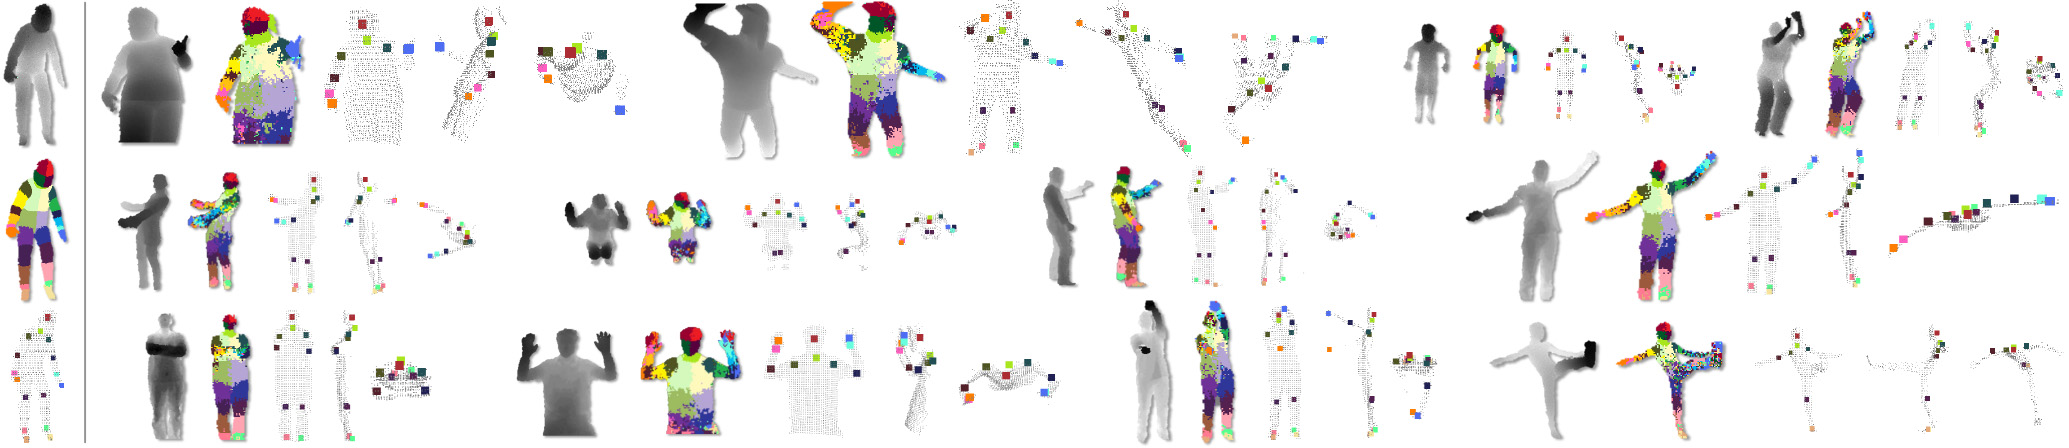
\includegraphics[width=160mm]{figures/content/ni-pose.jpg} \caption{Joint proposals are derived for various poses. Results of synthetic training data is shown on the top row, real training data shown in the middle row and failure modes at bottom. Left column shows a neutral pose as a reference. \cite{13} } \label{fg:ni:pose} 
\end{figure}


\paragraph*{Joints Proposal} Figure \ref{fg:ni:pose} shows example results of synthetic and real datasets. In each example we see the depth image, the derived label of most likely body part, and the front, right, and top views of the joint proposals overlaid on a depth point cloud.

\paragraph*{Skeletal points} Finally, the API returns positions and orientations of the skeleton joints as shown in the figure \ref{fg:ni:joints}. As well as, it returns the lengths of the body segments such as the distance between elbow and shoulder. Joint positions and orientations are given in the real world coordinate system. The origin of the system is at the sensor. +X points to the right, +Y points upward, and +Z points in the direction of increasing depth. 

\begin{figure}
	[h]
	\centering
	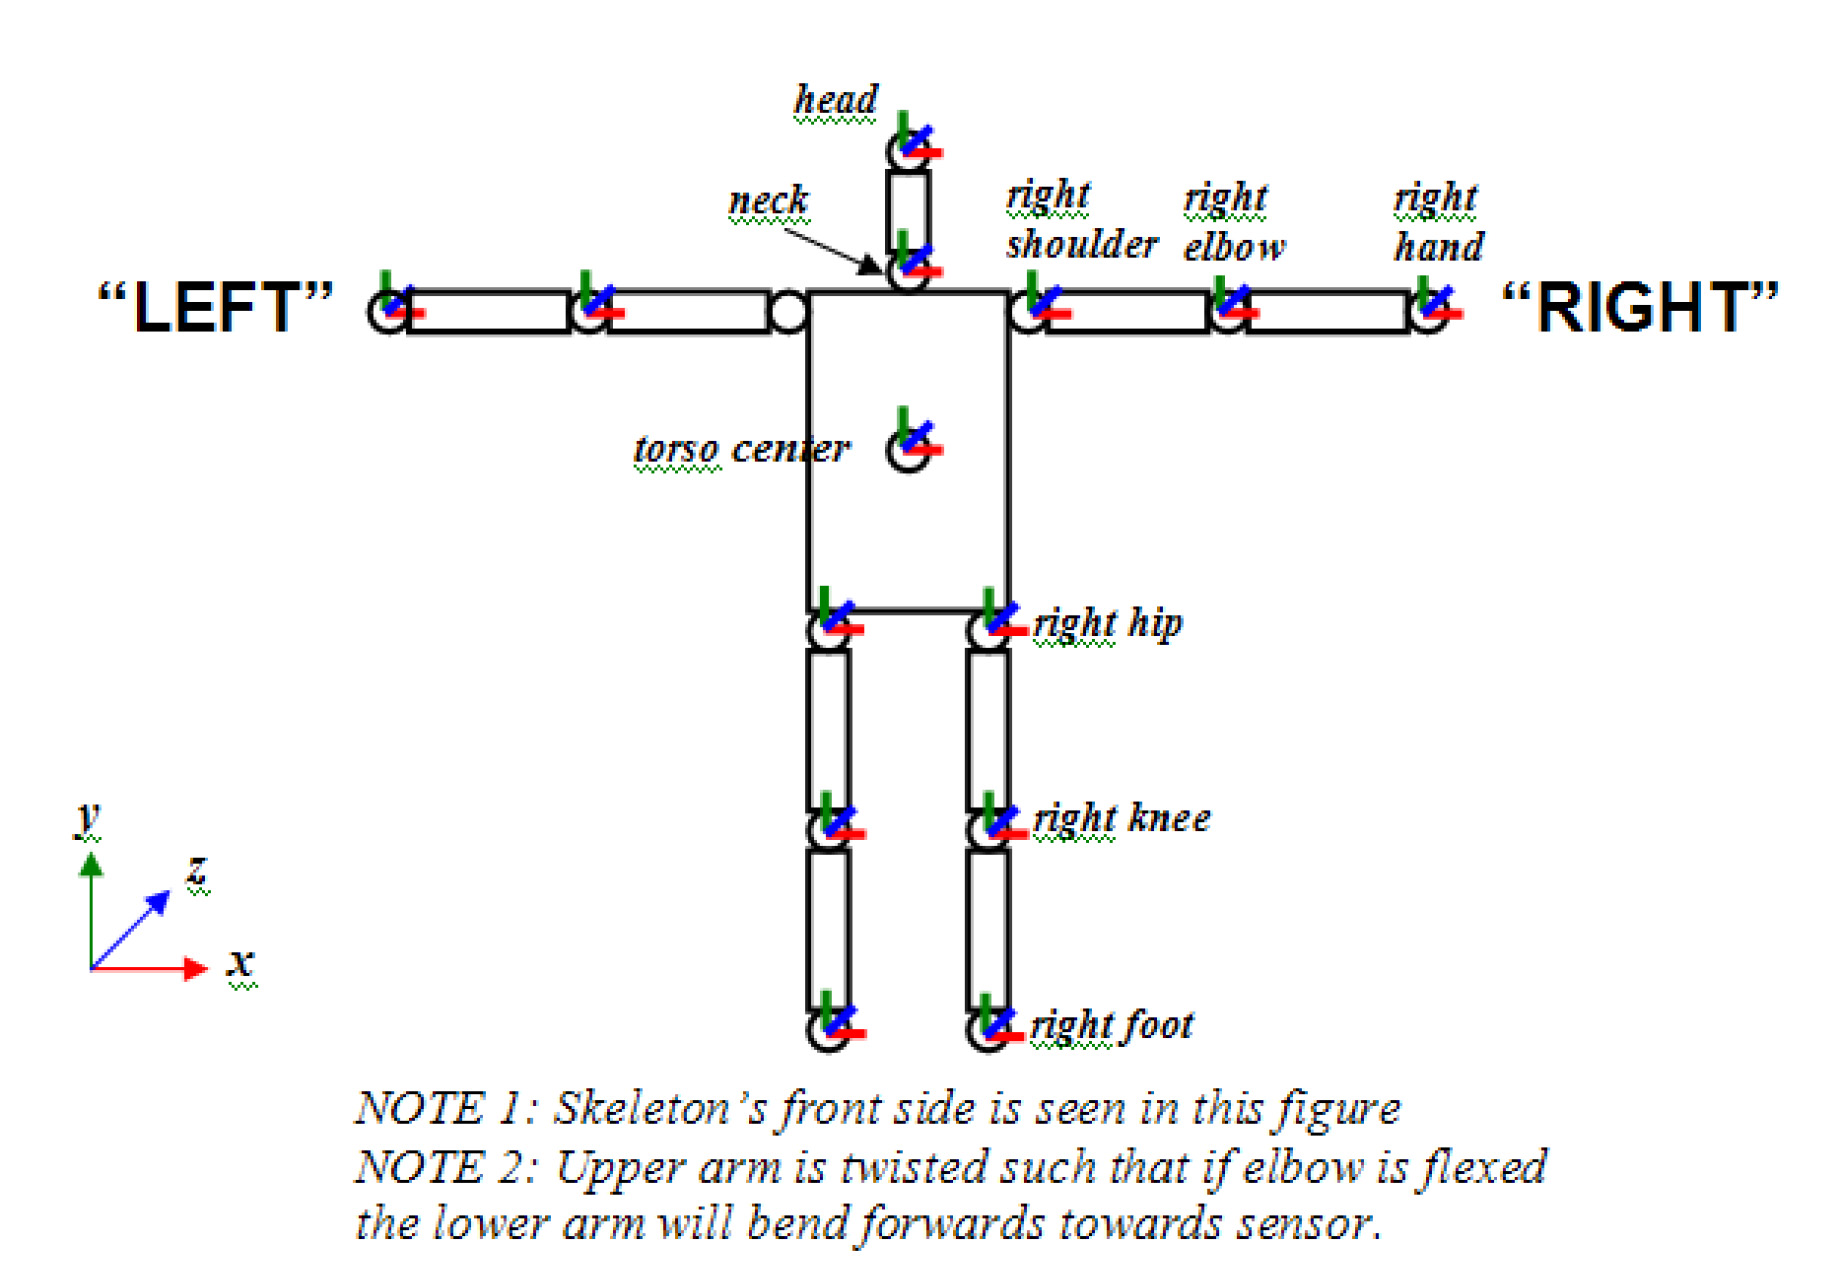
\includegraphics[height=10cm]{/content/ni-joints.jpg} \caption{Positions and orientations of the tracked skeleton return by NiTE API. \cite{12}} \label{fg:ni:joints} 
\end{figure}


\begin{figure}
	\centering 
	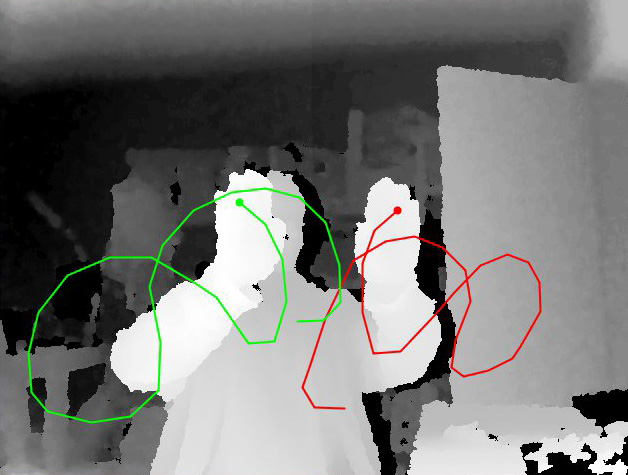
\includegraphics[height=8cm]{/content/ni-hand.jpg} \caption{NiTE Hand Tracking application shows the trail of the tracked hand in different colors. \cite{12} } \label{fg:ni:hand} 
\end{figure}


\paragraph*{Hand Tracker} Even though NiTE framework can recognize full human body, in this thesis we attempt to use only hand recognition and tracking due to the computational limitation of NAO described in the chapter \ref{ch:solution}. To start tracking a hand, a focus gesture must be gesticulated. There are two supported focus gestures: CLICK and WAVE. In the CLICK gesture, the user should hold the hand up and push it towards the sensor, then immediately pull the hand backwards. In the WAVE gesture, the user should hold the hand up and move it several times from left to right and back. Once hand is been found and it will be tracked till the hand leaves the field of view of the camera or hand point is lost due to various factors such as hand is touching another object or closer to another body part. Figure \ref{fg:ni:hand} shows how hand points are tracked using NiTE and trail of the hand positions in real world coordinates are mapped on to the depth image.

\paragraph*{Focus gestures} Focus gestures of NiTE is can be detected even during hand tracking session. NiTE gestures are derived from a stream of hand points thats records how a hand moves through space over time. Each hand point is at the center of the hand in real-world 3D coordinate measured in millimeters. Gesture detectors are sometimes called point listeners (or point controls) since they analyze the points stream looking for a gesture. NiTE recommends users to follow these suggestions to gain maximum efficiency from its API for Hand tracking.
\begin{itemize}
	\item Try to keep the hand that performs the gesture at a distance from your body. 
	\item Your palm should be open, fingers pointing up and face the sensor. 
	\item The movement should not be too slow or too fast. 
	\item WAVE should consist of at least 5 horizontal movements left-right or right-left. 
	\item CLICK should be long enough at least 20 cm and performed towards the sensor. 
	\item If you have difficulty in gaining focus, try to stand closer to the sensor (around 2m) and make sure that your hand is inside the field of view. 
\end{itemize}
